\begin{comment}
    %Con muchisimo dolor, esto se queda afuera de la tesis

    \subsection{Variable Elimination} \label{subSection:variableEliminationAlgorithm}

A continuación vamos a ver una explicación un poco más detallada del algoritmo \emph{Variable Elimination}. La operación de inferencia que queremos realizar con el mismo es $P(X_q \mid X_{e_1} = v_1 \land \ldots \land X_{e_j} = v_j)$, siendo $X_{e_1} = v_1 \land \ldots \land X_{e_j} = v_j$ la evidencia introducida en la red y las $X_{o_i} \neq X_q$ con $o_i \neq e_k$ nuestras variables ocultas. Primero descomponemos esta query en una sumatoria y multiplicación de probabilidades condicionales, basándonos en las dependencias de nuestra red bayesiana. Una vez que tenemos una sumatoria del estilo $\sum_{X_{h_1}} \ldots \sum_{X_{h_j}} P(..| ..) \ldots P(..| ..)$ nuestro algoritmo consiste en:  

\begin{enumerate} \label{alg:variableElimination}
    \item \textbf{Construir} un factor para cada distribución de probabilidad condicional.
    \item \textbf{Restringir} las variables observadas a sus valores observados.
    \item \textbf{Eliminar} cada variable oculta $X_o$:
    \begin{itemize}
        \item \textbf{Multiplicar} todos los factores que contienen $X_o$ para obtener un nuevo factor $g_j$.
        \item \textbf{Sacar} la variable $X_o$ del factor $g_j$ mediante suma.
    \end{itemize}
    \item \textbf{Multiplicar} los factores restantes.
    \item \textbf{Normalizar} el factor resultante, para que las probabilidades sumen 1.
\end{enumerate}

\santi{Estos itemizes generan un monton de duda ¿Qué es un factor? ¿Cómo es lo de eliminar una variable oculta?}

Su complejidad es polinomial basándose en la cantidad de variables y exponencial en base al tamaño de su mayor factor (siendo el tamaño la cantidad de variables del mismo). No podemos hacer algo mejor que la exponencial en el tamaño, pues el tamaño de una CPT de una variable de la red bayesiana $\aBayesianNetwork$ está dado por $O(c^f)$, siendo $c$ la cardinalidad máxima de una variable y $f$ la cantidad de variables en el factor. Por lo tanto, en principio $VE$ sería polinomial en el tamaño de $\aBayesianNetwork$, puesto que las operaciones de construir, restringir, multiplicar, remover y normalizar son polinomiales en base al tamaño. Dado que además la cantidad de nuevos factores que vamos a introducir son $O(n)$, con $n$ la cantidad de variables de $\aBayesianNetwork$.

%\santi{El tamaño no es en realidad $O(\sum_{v \in N} c_v^{f_v})$ donde $c_v$ es la cardinalidad del nodo $v$ y $f$ su cantidad de padres?} Echu: Noup, porque acá estoy hablando de una CPT individual de una variable, esa cota sería para todas las CPT's. Reformule la oración porque no se entendía eso. 

Pero tenemos un problema, en el tercer paso al eliminar la variable oculta $X_o$ puede ser que el nuevo factor $g_j$ sea mayor que todos los factores originales de $\aBayesianNetwork$, en ese caso la complejidad puede no ser polinomial. Al tamaño máximo de los nuevos factores $g_j$ se le llama ancho de eliminación (\emph{elimination width}). Esta medida se relaciona con el \emph{tree width}, puesto que el mejor \emph{elimination width} que uno puede obtener para los $n!$ órdenes posibles de eliminación de $\aBayesianNetwork$ es el \emph{tree width}. A raíz de esto es que se define la complejidad de este algoritmo como exponencial en el \emph{tree width} de $\aBayesianNetwork$, siendo esta $O(n*c^{ew})$, con $n$ la cantidad de variables, $c$ la cardinalidad máxima de una variable y $ew$ el ancho de eliminación. 

Igualmente, un valor acotado de $ew$ no alcanza, ya que encontrar el orden óptimo de eliminación es un problema \NP{-hard} \cite{orderingNpHard}, por lo que podría ser que encontrar este orden tampoco sea posible en tiempo polinomial. 

La complejidad de este algoritmo fue estudiada en varios artículos, por ejemplo en \cite{peyrard2018exactapproximateinferencegraphical} muestran distintos tipos de grafos en los cuáles \emph{Variable Elimination} (VE) puede realizarse en tiempo polinomial. Los \emph{polytrees} son uno de estos casos, ya que el orden de eliminación óptimo se puede encontrar en tiempo polinomial, el cuál corresponde al inverso del orden topológico. Puesto que en cada paso de la eliminación la cantidad de vecinos de ese nodo va a ser 1, por lo que su \emph{elimination width} va a ser 1, y por lo tanto la ejecución del algoritmo va a tardar un tiempo polinomial en el tamaño de la red. Por lo que la familia de grafos 
 %Ver si tiene sentido poner las explicaciones, ejemplos y dibujos del paper peyrard2018exactapproximateinferencegraphical, que la verdad están muy buenas. 
 %RTA Cifu: Ya está quedando muy larga, no agreguemos cosas que no suman tanto. 

\end{comment}
 

\subsection{Fórmulas }

\subsubsection{Funciones auxiliares del cálculo de los unrelated trees} \label{subsubSection:auxiliaryFormulasUnrelatedTrees}

Está es la definición de la función \textit{union} utilizada en la Ecuación \ref{formula:unrelated_equiv_classes}:

\begin{align}\label{formula:union}
&\union(((repEC_1, lTopo_1, rTopo_1), ...., (repEC_{|n|}, lTopo_{|n|}, rTopo_{|n|})), n_t) = \nonumber \\ 
&\left(\bigcup_{j=1}^{|n|} repEC_j \cup \set{n_t}, \binom{\sum_{i=1}^{|n|} |L(repEC_i)|}{|L(repEC_1)|, \ldots, |L(repEC_{|n|})|} \prod_{i=1}^{|n|} lTopo_i,\binom{\sum_{i=1}^{|n|} |R(repEC_i)|}{|R(repEC_1)|, \ldots, |R(repEC_{|n|})|} \prod_{i=1}^{|n|} rTopo_i \right)
\end{align}

La función $\union$ está definida en la Ecuación~\ref{formula:union}, y es la encargada de unir las distintas clases de equivalencia de los hijos de un nodo $n$. Más formalmente, $\union(n, ((repEC_1, lTopo_1, rTopo_1), \ldots)$ es la clase de equivalencia que se representa con $repEC$ en la cual el nodo $n$ está a la izquierda de $x_i$ y es compatible con las clases $repEC_i$ (en el sentido de que si un nodo aparece a la izquierda en $repEC_i$ entonces este también aparece a la izquierda en $repEC$, y de la misma forma con los que aparecen a la derecha). Para calcular la cantidad de órdenes topológicos a la izquierda y a la derecha de la clase utilizamos una fórmula muy similar a \ref{for:topoCountingDTrees}. Se puede aplicar la misma lógica porque no hay dependencias entre los nodos de los árboles no relacionados y sus subárboles, por lo que podemos combinar los órdenes topológicos sin restricciones.

\paragraph{Complejidad temporal de $union$}

$\union$ realiza 4 operaciones de costo $O(n)$ (pues $d_{out}(node)<n)$, 2 $\prod \ y \ \sum$. El coeficiente multinomial\footnote{Utilizamos el modelo de 
memoria RAM teniendo en cuenta que los factoriales pueden estar precalculados y que multiplicar números es $O(1)$ más allá de su tamaño. Igualmente, si el multinomial tomara $O(n^2)$, la complejidad total seguiría siendo la misma.} tiene costo $O(n)$, por lo que $\union$ tendrá una complejidad temporal de $O(n)$.



\subsubsection{Función completa de \leftPossibleOrders} \label{subsubSection:leftOrdersImplementation}

A continuación vamos a ver la implementación del algoritmo descrito en la sección \ref{alg:leftOrdersAlgorithm}. Los parámetros de la función serán:
\begin{itemize}
    \item $p$: posición en la que se colocó el último ancestro.
    \item $i$: índice del ancestro que vamos a colocar.
    \item $nodesPerAncestor$: una lista que contiene en la  $i$-ésima posición el número de nodos a la izquierda del unrelated tree de $a_i$.
        \begin{itemize}
            \item Debido a la ligera mejora mencionada en la sección \ref{slight_improvement}, solo habrá un árbol debajo de cada $a_i$, ya que si hay más de uno, estos árboles serán fusionados en uno solo. 
        \end{itemize}
\end{itemize}

Estas son las funciones auxiliares que vamos a utilizar:
\begin{itemize}
    \item $\mathrm{possibleCombinations}(l,i,nodesPerAncestor) \ \text{o} \ pb$, que devuelve todas las formas posibles de sumar $l$, utilizando los nodos de los primeros $i$ elementos de $nodesPerAncestor$.
        \begin{itemize}
            \item Por ejemplo, $\mathrm{possibleCombinations}(5,3,[4,2,1,7,\dots])= [[4,0,1], [4,1], [3,1,1], [3,2], [2,2,1]]$.
        \end{itemize}
    \item $\mathrm{hasPlaced}(placedNodes, nodesPerAncestor) \ \text{o} \ hp$, que devuelve una lista $l$ que tiene en la posición $i$-ésima el elemento $l[i]= nodesPerAncestor[i] - placedNodes[i]$. Lo que hace es restar de $nodesPerAncestor$ los elementos que ya colocamos en $placedNodes$.
    \item $\mathrm{canPlace}(i ,nodesPerAncestor) \ \text{o} \ cp$, que devuelve la suma de los primeros $i$ elementos de $nodesPerAncestor$.
\end{itemize}
Teniendo en cuenta estas funciones, la fórmula\footnote{Pueden encontrar este algoritmo en \path{\pasantia-BICC\asvFormula\classesSizes\recursiveFormula.py}} que vamos a utilizar para calcular los posibles ordenamientos de los nodos de las distintas clases de equivalencia de cada subárbol es:

%\label{formula:left_possible_orders}

 \[
    \leftPossibleOrders(p,i,npa) = 
    \begin{cases} 
    \begin{aligned}
        \binom{ cp(i, npa)}{npa[1], \ldots, npa[i]} 
    \end{aligned} & \text{if $|A|=i$} \\
    \begin{aligned}
    &\sum_{toFill=p}^{p+cp(i,npa)} \sum_{comb \in pb(toFill-p-1,i, npa)} \Big(\binom{ sum(comb)}{comb_1, \ldots, comb_i} \\
    &  \cdot \leftPossibleOrders(toFill,i+1,hp(comb, npa)\Big)
    \end{aligned}
    & \text{otherwise}
    \end{cases}
\]

%\echu{ Esto en realidad es más complejo, hay algunas transformaciones que se tienen que hacer a left. ¿Las anoto o no tiene sentido? (Es lo que se hace en leftElementsOfClasses en el código)} Rta: No hace falta, ya es suficientemente compleja la explicación y esa información no suma a entender el algoritmo

Nuestro caso base es cuando ya hemos colocado todos los ancestros, por lo tanto solo queda combinar los nodos que nos quedan por colocar. Luego, en el caso recursivo, él $toFill-p-1$ es el número de posiciones que necesitamos llenar entre el $a_i$ que estamos colocando y el $a_{i-1}$ que se colocó antes. En cada paso realizamos la sumatoria de cada posible combinación $comb$ de los elementos de $npa$, teniendo en cuenta todas las posibilidades de la cantidad de posiciones a llenar $toFill$ entre $a_i$ y $a_{i-1}$. Las posiciones van desde $p$ hasta $p$ más la máxima cantidad de nodos que podemos colocar ($cp(i,npa)$). Ahora, con todas estas funciones definidas, la llamada que resolverá $leftOrders(A, left)$ será $\leftPossibleOrders(0,0,left)$.

Para entender un poco cómo funciona este algoritmo veamos cuál podría ser un paso del mismo. En la Figura \ref{fig:leftOrdersIterationTopoOrder} podemos ver cómo sería el estado actual de los órdenes topológicos que estamos contando, teniendo en cuenta las decisiones previas que tomamos. Los nodos pintados en naranja que vemos en la Figura \ref{fig:leftOrdersIterationGraph} son los nodos que tenemos disponibles para rellenar ese espacio en rojo. En cambio, los nodos de $u_i$ no los podemos utilizar todavía, ya que todavía no colocamos el nodo $a_i$. Una vez que lo coloquemos podremos utilizarlos. 

%\echu{ Hace falta agregar un dibujo o ilustración para que el algoritmo quede más claro?}
%\%sergio{Creo que vendría muy bien}

\begin{figure}[ht]
    \centering
    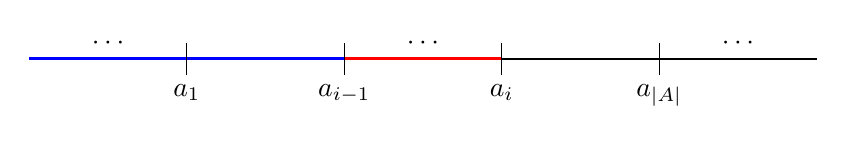
\begin{tikzpicture}
        % Línea principal
        \draw[thick] (0,0) -- (10,0);

        % Segmento azul: inicio -> a_{i-1}
        \draw[blue, very thick] (0,0) -- (4,0);

        % Segmento rojo: a_{i-1} -> a_i
        \draw[red,  very thick] (4,0) -- (6,0);
        
        % Marcas y etiquetas
        \foreach \x/\etiqueta in {2/$a_1$, 4/$a_{i-1}$, 6/$a_i$, 8/$a_{|A|}$} {
            \draw (\x,0.2) -- (\x,-0.2);          % ticks
            \node[below] at (\x,-0.2) {\etiqueta}; % etiquetas
        }

        % Puntos suspensivos
        \node at (1,0.2) {$\cdots$};
        \node at (5,0.2) {$\cdots$};
        \node at (9,0.2) {$\cdots$};
    \end{tikzpicture}
    \caption{$i$-ésimo paso de \leftPossibleOrders. La línea azul son los nodos ya colocados y la línea roja tiene longitud $toFill-p-1$, definiendo el espacio que hay para colocar los nodos disponibles.}
    \label{fig:leftOrdersIterationTopoOrder}
\end{figure}


\begin{figure}[H]
    \centering
    \begin{tikzpicture}[scale=.65, transform shape, 
    unrelated/.style={circle, draw=red},
    ancestor/.style={circle, draw=blue},
    wiggly/.style={decorate, decoration={snake, amplitude=.2mm, segment length=2mm}}  % Define wiggly line style
    ]

        \node[draw=none, fill=none] (a1) at (0, 0) {};
        \node[ancestor] (a2) at (1, -2) {$a_{i-1}$};

        \drawUnrelatedTreeWithTag{u2}{-1}{-4}{$u_{i-1}$}{orange}{Available nodes: npa[i-1]}

        \drawUnrelatedTree{u4}{0}{-7}{$u_{i}$}
        \node[ancestor] (a3) at (3, -6) {$a_i$};

        \node[draw=none, fill=none] (xi) at (3, -8) {};

        \drawUnrelatedTreeWithTag{r1}{6}{0}{$u_5$}{orange}{Available nodes: npa[0]};
        \drawUnrelatedTreeWithColor{r2}{10}{0}{$u_6$}{orange};


         \path [->] (a1) edge[arista,  decorate, decoration={snake, amplitude=.4mm, segment length=4mm, post length=1mm}] (a2);

         \path [->] (a2) edge[arista]  (u2);
         \path [->] (a2) edge[arista]  (a3);

         \path [->] (a3) edge[arista]  (u4);
         \path [->] (a3) edge[arista,  decorate, decoration={snake, amplitude=.4mm, segment length=4mm, post length=1mm}] (xi);
    \end{tikzpicture}
    \caption{Los nodos pintados en naranja son los nodos disponibles para ser colocados en el paso $i$. Para cada conjunto de subárboles $npa$ tiene la cantidad de nodos disponibles.}
    \label{fig:leftOrdersIterationGraph}
\end{figure}


\paragraph{Complejidad temporal de $\leftPossibleOrders$}
Analicemos la complejidad temporal de $\leftPossibleOrders$, para obtenerla necesitamos saber cuánto cuesta calcular cada nodo y cuántos estados posibles hay. %, ya que estamos utilizando programación dinámica. 

Comencemos con los estados posibles. Tenemos los parámetros $i$, $p$ y $nodesPerAncestor$. El índice $i$ tiene $|A|$ valores posibles, con $|A| \in O(n)$. Luego $p$ puede tomar $O(n)$ valores posibles, debido a que un orden topológico puede tener como máximo $n$ nodos. Ahora tenemos que calcular el número de estados posibles para $nodesPerAncestor$.

Para cada posición $npa[i]$ vamos a tener el número de nodos a la izquierda de los unrelated trees bajo $a_i$. Definimos $size(ut_i)$ el tamaño del unrelated tree $ut_i$ bajo el nodo $a_i$ (si no hay ninguno, es 0). Para la posición $i$-ésima, tenemos $size(ut_i)$ valores posibles. Por la Fórmula \ref{formula:number_of_equiv_classes}, sabemos que $\numEqCl(ut_i) > size(ut_i)$, por lo que los valores posibles de $nodesPerAncestor$ están acotados por $\prod_{i=0}^{|A|} size(ut_i) < \prod_{i=0}^{|A|} \numEqCl(ut_i)$ (esta es la combinatoria de cada valor posible en cada posición). Utilizando la Fórmula \ref{formula:number_of_equiv_classes}, sabemos que $\prod_{i=0}^{|A|} \numEqCl(ut_i) < |equivalenceClasses|$, ya que la productoria de las clases de cada subárbol no puede ser mayor a la cantidad total de clases. Con eso, podemos concluir que los valores posibles de $npa$ \emph{están acotados por el número de clases de equivalencia}.

Entonces, concluimos que el número de estados de \leftPossibleOrders \ es $values(i) \cdot values(p) \cdot values(npa) \in O(n) \cdot O(n) \cdot |equivalenceClasses| = O(n^2 \cdot |equivalenceClasses|)$.

Queda ver cuánto cuesta computar cada nodo. El coeficiente multinomial toma $O(n^2)$, así que el número de sumas determinará nuestra complejidad. $toFill$ puede tomar como máximo $\sum_{j=0}^i nodesPerAncestor[j] \in O(n)$ valores en cada iteración. 

Resta determinar cuántos valores puede tomar $\mathrm{possibleCombinations}(l,i,nodesPerAncestor)$. Sabemos que para cada resultado $res$ tal que $res \in pb(l,i,npa)$ se cumple que $\forall 0<j<|res|, 0<res[j]<npa[j]$. Usando un argumento similar al de $nodesPerAncestor$, podemos concluir que $size(pb(l,i,npa)) < |equivalenceClasses|$. Así concluimos que el costo de calcular cada estado es $O(n \cdot |equivalenceClasses| \cdot n^2) = O(n^3 |equivalenceClasses|) $, que es la cantidad de iteraciones de la primera y segunda sumatoria, multiplicado por el costo de evaluar el multinomial. Por lo que finalmente la complejidad de calcular $leftSize$ es $O(|estados|)\cdot O(computarNodo)$ = $O(n^5 \cdot |equivalenceClasses|^2)$.

\subsubsection{Funciones auxiliares del cálculo de clases de equivalencias} \label{subsubSection:auxiliaryFormulasEquivalenceClasses}

\begin{align*}
eqClass(A, D, ((eqCl_1, \_ , \_ ), ...., (eqCl_{|UR|}, \_ , \_))) 
    &=  \set{a_l \mid a \in A} \cup \set{d_r \mid d \in D} \cup (\bigcup_{j=1}^{|UR|} eqCl_j) \\ 
\eqClassSize(A, D, mix) 
    &= leftSize(A,mix) \cdot rightSize(D, mix)  \\ 
leftSize(A, ((_, l_1, \_), ...., (_, l_{|UR|}, \_))) 
    &= leftOrders(A, [ l_1, \dots, l_{|UR}]) \cdot \prod_{i=1}^{|UR|} l_i  \\
rightSize(D, ((eqCl_1, \_, r_1), ...., (eqCl_{|UR|}, \_, r_{|UR|} ))) 
    &= \binom{|D| + \sum_{i=1}^{|n|} |R(eqCl_i)|}{|R(eqCl_1)|, \ldots, |R(eqCl_{|n|})|, |D|} \cdot \prod_{i=1}^{|UR|} r_i * \numTopo(x_i)
\end{align*}


En $eqClass$ obtenemos representación de la clase de equivalencia $\equivalenceClassRep$, colocando los nodos en $A$ antes de $x_i$m los nodos en $D$ después y dejando con el mismo tag los nodos de $mix$. En $\#eqClass$ obtenemos el tamaño de la clase de equivalencia, multiplicando todos los órdenes topológicos posibles de la izquierda por los de la derecha, ya que una combinación de ambos respetará la clase de equivalencia. Para $rightSize$ usamos la misma fórmula que antes y simplemente añadimos los órdenes topológicos de los descendientes utilizando la fórmula de \ref{for:topoCountingDTrees}. Y para $leftSize$ calculamos las posibles combinaciones usando la función que aparece a continuación.

\paragraph{Complejidad de \eqClassSize} \label{subsubSection:eqClassComplexity}

Primero, necesitamos calcular la complejidad temporal de $rightSize$, que es $O(n^2)$. Tenemos el coeficiente multinomial, que toma $O(n)$ tiempo , el $\prod$ que es $O(n)$, ya que $|UR|<n$ y $\numTopo(x_i)$ que puede implementarse en $O(n^2)$. Entonces, la suma de estas operaciones tiene complejidad $O(n^2)$.

%\santi{Antes dijiste $O(n^2)$}

Luego para $leftSize$ sabemos que la complejidad temporal del Algoritmo \ref{alg:leftOrdersAlgorithm} es de $O(n^5 \cdot |equivalenceClasses|^2)$. En la sección \ref{subsubSection:leftOrdersImplementation} del apéndice se encuentra la justificación de esta complejidad. 

Eso nos deja con una complejidad temporal de $O(n^5 \cdot |equivalenceClasses|^2)$ para $\eqClassSizes$, puesto que la complejidad de $rigthSize$ está acotada por la de $leftSize$.



\subsubsection{Complejidad de \texttt{allPossibleOrders}} \label{subsubSection:allPosibleOrdersComplexity}

El cálculo para obtener la complejidad de $allPosibleOrders$ es muy similar al hecho en \ref{subsubSection:eqClassComplexity} para \leftPossibleOrders, solo que ahora no tenemos las clases de equivalencia para acotar los valores. Así que tenemos que hacer las cuentas combinatorias para tener una complejidad en función del digrafo $D$. Al también usar dinámica vamos a tener que calcular la cantidad de estados y cuánto cuesta computar cada uno. 

Los valores que tenemos que tener en cuenta para nuestros estados son $nodeIndex, nodesBefore, nodesAfter$. 

El algoritmo \texttt{allPossibleOrders} utiliza programación dinámica con memoización. Su complejidad total se obtiene al multiplicar la cantidad de \emph{estados} posibles por el \emph{costo computacional por estado}.

Sean:
\begin{itemize}
    \item $k = d_{\text{in}}(v) + d_{\text{out}}(v) + 1$ el número total de vecinos (padres e hijos) del nodo actual más el propio nodo.
    \item $S$ la cantidad total de nodos a colocar, es decir, $S = \texttt{nodosRestantes} - k$.
\end{itemize}

\paragraph{Número de estados} Cada estado está definido por un índice $i \in [0, k]$ y  dos vectores de tamaño $k$: \texttt{nodesBefore}, \texttt{nodesAfter}, con entradas en $\mathbb{N}$ cuya suma total es $S$. La cantidad de formas de repartir $S$ unidades entre $2k$ casillas (coordenadas de los vectores \texttt{nodesBefore} y \texttt{nodesAfter}) es:
\[
\binom{S + 2k - 1}{S}
\]
Entonces, el número total de estados es $O\left(k \cdot \binom{S + 2k - 1}{S}\right).$

\paragraph{Costo por estado} Dentro de cada estado se generan todas las combinaciones posibles de distribuir $t \leq S$ nodos\footnote{En realidad no se tiene en cuenta hasta $S$, sino meramente los nodos que se pueden colocar en ese momento, pero utilizamos $S$ como cota. } entre hasta $k$ posiciones. Para cada $t$ hay $\binom{t + k - 1}{k - 1}$ combinaciones posibles. Luego por la identidad de la escalera se cumple que:
    \[
    \sum_{t=0}^{S} \binom{t + k - 1}{k - 1} = \binom{S + k}{k},
    \]
     Cada una de estas combinaciones se procesa en $O(k)$. Por lo tanto, el costo por estado es: $O\left(\binom{S + k}{S} \cdot k\right).$



\paragraph{Complejidad total}

Multiplicando la cantidad de estados por el costo por estado:

\[
T(S, k) = O\left(
    k^2\cdot
    \binom{S + 2k - 1}{S} \cdot
    \binom{S + k}{S}
\right).
\]

\paragraph{Casos particulares}

A continuación analizamos cómo se comporta la complejidad en función de los parámetros $S$ y $k$:

\begin{itemize}
    \item \textbf{Caso 1: $k$ constante (por ejemplo, $k = 3$)}.  
    Si el número de vecinos involucrados en la combinación es una constante fija, entonces los binomios
    \[
    \binom{S + 2k - 1}{S} \quad \text{y} \quad \binom{S + k}{S}
    \]
    se comportan como polinomios en $S$ de grado $2k - 1$ y $k$ respectivamente. Por lo tanto, la complejidad total se acota por un polinomio:
    \[
    T(S) = O\left(S^{3k - 1}\right),
    \]
    lo que resulta eficiente para instancias en las que el número de vecinos a combinar está acotado.

    \item \textbf{Caso 2: $k = O(n)$ y $S = O(n)$}.  
    En el peor caso, donde el nodo actual tiene un número lineal de vecinos (por ejemplo, si el grafo es muy denso o el nodo es central en la topología), tanto $k$ como $S$ pueden crecer linealmente con $n$. En este escenario, los coeficientes binomiales se comportan asintóticamente como:
    \[
    \binom{S + 2k - 1}{S} = \Theta\left( \frac{(3n)!}{n! \cdot (2n)!} \right),
    \qquad
    \binom{S + k}{S} = \Theta\left( \frac{(2n)!}{n! \cdot n!} \right),
    \]
    lo cual implica una complejidad exponencial. En particular:
    \[
    T(n) = O\left( n^2 \cdot \binom{3n}{n} \cdot \binom{2n}{n} \right),
    \]
    que es significativamente mayor que $n!$ y confirma que el algoritmo no es eficiente en este caso. 
\end{itemize}

%\echu{Acá estoy mintiendo un poco porque no estoy teniendo en cuenta a nodesToPutBefore, pero agrega un $*O(n)$ nada más y me obligaría a explicar más en detalle la función. ¿Puedo ignorarlo y utilizar sólo los otros dos para hacer las cuentas?}


\subsection{Demostraciones}

\subsubsection{ASV puede calcularse en tiempo polinomial para una distribución Naive Bayes} \label{subsubSection:proofASVPolynomialNaiveBayes}

\begin{theorem}
Los Asymmetric Shapley Values pueden calcularse en tiempo polinomial para distribuciones dadas como una Red Bayesiana Naive y para una familia de modelos \(\mathcal{F}\) si y solo si los Shapley values pueden calcularse para la familia \(\mathcal{F}\) bajo una distribución producto arbitraria en tiempo polinomial.
\end{theorem}

\begin{proof}
Primero, probamos la implicación de derecha a izquierda. Sea \(x_1\) el padre de todos los demás nodos en el DAG. Vamos a mostrar cómo calcular \(\assym_{M,e,\Pr}(x_j)\) para cualquier \(2 \leq j \leq n\) y \(\assym_{M,e,\Pr}(x_1)\) de forma independiente.

Observemos que el DAG tiene \((n-1)!\) órdenes topológicos, uno para cada permutación de los features \(\{x_2, \ldots, x_n\}\), y \(\pi(x_1) = 1\) para todas ellas. Entonces,

\[\label{eq:assymetric_for_naive_child}
\assym_{M,e,\Pr}(X_j) = \sum_{\pi \in \topo(G)} w(\pi) \left[ \charactheristicFunction_{M,e,\Pr}(\pi_{<j} \cup \{x_j\}) 
- \charactheristicFunction_{M,e,\Pr}(\pi_{<j}) \right]
\]

es equivalente a:

\[
\assym_{M,e,\Pr}(X_j) = \frac{1}{(n-1)!} \sum_{\pi \in \perm(\{x_2, \ldots, x_n\})} \left[ \charactheristicFunction_{M,e,\Pr}(\{x_1\} \cup \pi_{<j} \cup \{x_j\}) - \charactheristicFunction_{M,e,\Pr}(\{x_1\} \cup \pi_{<j}) \right]
\]

Así, una vez que \(x_1\) está fijado, la distribución para las variables \(x_2, \ldots, x_n\) es una distribución producto con \(p_{x_j} = P(X_j = 1 | X_1 = e(x_1))\). Para simplificar, asumamos que \(e(x_1) = 1\), y consideremos la distribución de producto \(\Pr'\) definida como:

\[
\Pr\,'[X_i = 1] = p_i = 
\begin{cases}
1 & i = 1 \\
\Pr[X_i = 1 | X_1 = e(x_1)] & \text{en otro caso}
\end{cases}
\]

que intuitivamente se obtiene de \(\Pr\) fijando \(X_1 = 1\). Siempre que \(x_1\) esté fijo, ambas distribuciones \(\Pr\) y \(\Pr'\) se comportan de la misma forma:


\begin{lemma}\label{lemma:valuation_of_prob_function}
Para cualquier \(S \subseteq X \setminus \{x_1\}\), se cumple que:
\[
\charFunML_{M,e,\Pr}(\{x_1\} \cup S) = \charFunML_{M,e,\Pr'}(\{x_1\} \cup S) = \charFunML_{M,e,\Pr'}(S)
\]
\end{lemma}

\begin{proof}
Esto se sigue de directamente manipulando la expresión:
    
    \begin{align}
        \charFunML_{M,e,\Pr}(\{x_1\} \cup S) &= \sum_{e' \in \consistsWith(e,\{x_1\} \cup S)} \Pr[e' | S] M(e') \nonumber \\
        &= \sum_{e' \in \consistsWith(e, \{x_1\} \cup S)} \left( \prod_{\substack{e'(y) = 1 \\ y \notin \{x_1\} \cup S}} p_y \prod_{\substack{e'(y) = 0 \\ y \notin \{x_1\} \cup S}} (1-p_y)\right) M(e')\\
        &= \sum_{e' \in \consistsWith(e, S)} \left( \prod_{\substack{e'(y) = 1 \\ y \notin S}} p_y \prod_{\substack{e'(y) = 0 \\ y \notin S}} (1-p_y)\right) M(e') \nonumber\\
        &= \sum_{e' \in \consistsWith(e, S)} \Pr\,'[e' | S] M(e') \nonumber\\
        &= \charFunML_{M,e,\Pr'}(S) \nonumber
    \end{align}
    
    donde la segunda igualdad viene de reemplazar $Pr$ por la distribución producto y la tercera igualdad se deduce al observar que para todas las entidades $e' \in \consistsWith(e, S)$ tales que $e'(x_1) = 0$ se cumple que 
    
    $$\prod_{\substack{e'(y) = 1 \\ y \notin S}} p_y \prod_{\substack{e'(y) = 0 \\ y \notin S}} (1-p_y) = 0$$
    
    Además, la segunda ecuación es igual a $\charFunML_{M,e,\Pr'}(\{x_1\} \cup S)$.
    \end{proof}

    
%TODO: Seguir repasando esta demo y ver de entenderla bien de pi a pa
    Usando este lema, ahora demostramos
    
    \begin{align}\label{eq:relation_between_assym_and_shap_naive_child}
        \assym_{M,e,\Pr} (x_j) = \Shap_{M,e,\Pr'}(x_j)
    \end{align}
    
    Se cumple que %\sidesergio{Super menor, pero quizás en estas circunstancias siempre poner dos puntos:, o nunca}
    
    \begin{align*}
        \Shap_{M,e,\Pr'}(x_j) &= \frac{1}{n!} \sum_{\pi \in \perm(X)} \left[ \charFunML_{M,e,\Pr'}(\pi_{<j} \cup \{x_j\}) - \charFunML_{M,e,\Pr'}(\pi_{<j}) \right]\\
        &= \frac{1}{n!} \sum_{\pi \in \perm(X)} \left[ \charFunML_{M,e,\Pr'}(\{x_1\} \cup \pi_{<j} \cup \{x_j\}) - \charFunML_{M,e,\Pr'}(\{x_1\} \cup \pi_{<j}) \right]\\
        &= \frac{n}{n!} \sum_{\pi \in \perm(\{x_2,\ldots,x_n\})} \left[ \charFunML_{M,e,\Pr'}(\{x_1\} \cup \pi_{<j} \cup \{x_j\}) - \charFunML_{M,e,\Pr'}(\{x_1\} \cup \pi_{<j}) \right] \\
        &= \frac{1}{n-1!} \sum_{\pi \in \perm(\{x_2,\ldots,x_n\})} \left[ \charFunML_{M,e,\Pr}(\{x_1\} \cup \pi_{<j} \cup \{x_j\}) - \charFunML_{M,e,\Pr}(\{x_1\} \cup \pi_{<j}) \right]\\
        &= \assym_{M,e,\Pr}(x_j)
    \end{align*}
    
    donde la segunda y cuarta igualdad se siguen del Lema~\ref{lemma:valuation_of_prob_function}, la última igualdad de la Ecuación~\ref{eq:assymetric_for_naive_child} y la tercera al observar que para cada permutación de $\perm(\{x_2,\ldots,x_n\})$ podemos construir $n$ permutaciones de $\perm(X)$ insertando $x_1$ en todos los lugares posibles, y que para cada una de estas permutaciones la expresión dentro de la suma es la misma. Así, la Ecuación~\ref{eq:relation_between_assym_and_shap_naive_child} muestra que calcular $\assym_{M,e,\Pr}(x_j)$ se reduce a calcular los valores Shapley habituales para una distribución independiente particular.
    
    Ahora consideramos $\assym_{M,e,\Pr}(x_1)$. Observemos que
    
    \begin{align*}
        \assym_{M,e,\Pr}(x_1) &= \frac{1}{|\topo(G)|} \sum_{\pi \in \topo(G)} \left[ \charFunML_{M,e,\Pr}(\pi_{<1} \cup \{x_1\}) - \charFunML_{M,e,\Pr}(\pi_{<1}) \right]\\
        &= \frac{1}{|\topo(G)|}( \charFunML_{M,e,\Pr}(\{x_1\}) - \charFunML_{M,e,\Pr}(\emptyset))
    \end{align*}

    %\echu{¿En esta fórmula de Shap no falta el $\frac{1}{|\topo(G)|}$? Porque sino no se estaría normalizando el resultado.}
    
    ya que para todas las permutaciones el conjunto $\pi_{<1} = \emptyset$. Además, sabemos que $\charFunML_{M,e,\Pr}(\{x_1\}) = \charFunML_{M,e,\Pr'}(\emptyset)$ por el Lema~\ref{lemma:valuation_of_prob_function}, y que
    
    \begin{align*}
        \charFunML_{M,e,\Pr}(\emptyset) &= \sum_{e' \in \entities(X)} \Pr[e] M(e)\\
        &= \sum_{\substack{e' \in \entities(X) \
        \ e'(x_1) = 1}} \Pr[e' | e'(x_1) = 1] \Pr[X_1 = 1] M (e') + \sum_{\substack{e' \in \entities(X) \\ e'(x_1) = 0}} \Pr[e' | e'(x_1) = 1] \Pr[X_1 = 0] M (e')\\
        &= \Pr[X_1 = 1] \charFunML_{M,e,\Pr'}(\emptyset) + \Pr[X_1 = 0] \charFunML_{M,e,\Pr''}(\emptyset)
    \end{align*}
    
    donde la distribución $\Pr''$ es la distribución producto obtenida al fijar $X_1 = 0$ como
    
    \begin{align*}
        \Pr \, ''[X_i = 1] = \begin{cases}
            0 & i = 0\\
            Pr[X_i = 1 | X_1 = 0] & \text{de otro modo}
        \end{cases}
    \end{align*}
    
    Finalmente,
    
    \begin{align*}
        \assym_{M,e,\Pr}(x_1) = \frac{1}{|\topo(G)|}( (1 - \Pr[X_1 = 1]) \charFunML_{M,e,\Pr'}(\emptyset) - \Pr[X_1 = 0] \charFunML_{M,e,\Pr''}(\emptyset))
    \end{align*}
    
    y reducimos el problema de calcular $\assym_{M,e,\Pr}(x_1)$ al de calcular la predicción promedio del modelo $M$ para dos distribuciones independientes diferentes $\Pr'$ y $\Pr''$. Según \cite{van2022tractability}[Teorema 1], se cumple que estos promedios pueden ser calculados en tiempo polinomial si y sólo si los valores de Shapley pueden ser calculados en tiempo polinomial para una distribución de producto arbitraria.
    
    La demostración de izquierda a derecha sigue al observar que una distribución producto es un caso particular de una Distribución Naive Bayes en la cual, para cualquier valor del padre $X_1$, las distribuciones condicionales son las mismas.

    %\echu{ ¿Debería escribir la demo de izquierda a derecha? ¿O inecesario? No se si tiene mucho sentido, ya está muy pesada la tesis} Rta: No hace falta, con esto alcanza. 
        
    \end{proof}

\subsubsection{Cota superior para la cantidad de clases de equivalencia} \label{subsubSection:proofUpperBoundEquivalenceClasses}

\begin{lemma}
    Para cualquier árbol $T$, donde $l$ es el número de hojas y $h$ es la altura para la raíz $n$ de $T$. Entonces, para la fórmula: 
    \[
    \numEqCl(n) = 
    \begin{cases} 
    2 & \text{if $n$ is a leaf} \\
    \prod_{c \in children(n)} \numEqCl(c) + 1 & \text{oc.}
    \end{cases}
    \]
    Tenemos la cota $\numEqCl(n) \leq h^{l} + 1$
      
\end{lemma}

\begin{proof}
    Queremos demostrar que $\numEqCl(n) \leq h_n^{l_n} + 1$. Esto aplica a cualquier árbol $T$ y su raíz $n$, donde $l_n$ es el número de hojas del árbol y $h_n$ es su altura.

    Debemos demostrar esto para los dos casos que presenta la fórmula.

    \textbf{Caso 1: $n$ es una hoja}
    Si $n$ es una hoja, entonces tiene altura 1, y su número de hojas es 1. Esto nos deja con $\numEqCl(n) = 2 \leq  2 = (1)^1 + 1$. 

    \textbf{Caso 2: $n$ tiene hijos}

    Nuestra \textit{hipótesis inductiva} es que para cada subárbol $T_h$ que tiene un hijo $c$ de $n$ como raíz, nuestra fórmula se cumple. Esto significa que $\forall c \in children(n), \numEqCl(c) \leq h_c^{l_c} + 1$. Con esto en mente, veamos que
\begin{align*}
    \numEqCl(n)  
        &= (\prod_{c \in children(n)} \numEqCl(c)) + 1 \\
        &\leq (\prod_{c \in children(n)} h_c^{l_c} + 1) + 1 \\
       &\leq \prod_{c \in children(n)} h_n^{l_c} + 1 \\
        &= h_n^{\sum_{c \in children(n)} l_c} + 1 \\
        &= h_n^{l_n} + 1 
\end{align*}


    %\santi{No es muy estándar esto de poner entre paréntesis el motivo de la simplificación después de la desigualdad. Capaz es más común ponerlo al fondo a la derecha en la misma línea (como si fuera un comentario de código)}
    En la primera desigualdad aplicamos la hipótesis inductiva. Después, en la segunda desigualdad sabiendo que por la definición de altura se cumple $(\forall c \in children(n)) \ h_n = h_c + 1$, entonces $\forall k \in \mathbb{N}$ se cumple $h_n^k = (h_c + 1)^k \geq h_c^k + 1$. En la última igualdad utilizamos que $\sum_{c \in children(n)} l_c = l_n$).

    Así concluimos que nuestra fórmula tiene una cota superior de $h^l + 1$. 
\end{proof}

\subsubsection{Error para la estimación de ASV a través de sampleos} \label{subsubSection:proofErrorSamplingASV}

El siguiente lema nos permite ver que dado un mecanismo de sampleo de este tipo sería posible aproximar el ASV de forma eficiente.

\begin{lemma}[Estimación de ASV a través de sampleos]
    \label{theorem:asvSamplingError}

    Sea $M$ un modelo, $e$ una entidad, $G$ un grafo causal para el conjunto de features $X$ de $M$ y $\Pr$ una distribución sobre el conjunto de entidades. Supongamos que existe un algoritmo $\anAlgorithm$ que dado un subconjunto $S \subseteq X$ de features, calcula el valor $\nu_{M, e, \Pr}(S) =\mathbb{E}[M(e') | \consistsWith{}(e, S)]$. Supongamos también que existe un mecanismo $\aMechanism$ para samplear órdenes topológicos de $G$ de forma uniforme.

    Luego, dada una precisión $\varepsilon > 0$ y una probabilidad $\delta \in (0, 1)$, es posible estimar el ASV para un modelo $M$, una entidad $e$ y una feature $x$ con precisión $\varepsilon$ y probabilidad de error $1-\delta$ usando $O(\log(1-\delta)/\varepsilon^2)$ sampleos de $\aMechanism$ y $O(\log(1-\delta) / \varepsilon^2)$ llamados a $\anAlgorithm$.
    
\end{lemma}

\begin{proof}
    Veamos a $\aMechanism$ como una variable aleatoria distribuida uniformemente sobre 
    
    \begin{align*}
        T = \{\overline{x} \in \pi(X) : \overline{x} \text{ es un orden topológico de $G$}\}
    \end{align*}
    
    (es decir, sobre los órdenes topológicos de $G$). Luego, si definimos $g: T \to \mathbb{R}$ como

    \begin{align*}
        g(\overline{x}) = \nu_{M, e, \Pr}(\overline{x}_{<x} \cup \{x\}) - \nu_{M, e, \Pr}(\overline{x})
    \end{align*}

    tenemos que

    \begin{align}\label{eq:ASV_to_sample}
        ASV(M, e, x) = \frac{1}{|T|} 
        \sum_{\overline{x} \in T} g(\overline{x}) = \mathbb{E}[g(\aMechanism)]
    \end{align}

    Notemos que podemos samplear la variable $g(\aMechanism)$ sampleando primero $\aMechanism$ y luego usando el algoritmo $\anAlgorithm$.
    
    La ecuación \eqref{eq:ASV_to_sample} nos dice que podemos estimar el ASV estimando el valor $\mathbb{E}[g(\aMechanism)]$, el cual a su vez podemos estimar sampleando la variable $g(\aMechanism)$. Para obtener una cota a la cantidad de sampleos necesarios para obtener precisión $\varepsilon$ usaremos desigualdades tradicionales, como la de Hoeffding. La misma dice que dadas variables aleatorias $\{X_i\}_{1 \leq i \leq k}$ independientes e idénticamente distribuidas con valores en el rango $(a, b)$ se tiene que

    \begin{align*}
        P(|\sum_{i=1}^k X_i - \mathbb{E}[X_i]| \geq \varepsilon) \leq 2e^{-2\varepsilon^2k / (b-a)}
    \end{align*}

    En nuestro caso, la variable $g(\aMechanism)$ tiene valor en el rango $[-1, 1]$, por lo que podemos pedir que la probabilidad de error sea a lo sumo $1-\delta$ despejando la ecuación

    \begin{align*}
        2e^{-\varepsilon^2 k} \leq 1 - \delta
    \end{align*}

    , de lo cual se obtiene que

    \begin{align*}
        \frac{\log ((1 - \delta) / 2)}{e^2} \leq k
    \end{align*}

    Por lo tanto, haciendo $k = O(\log(1-\delta) / \varepsilon^2)$ sampleos se obtiene un estimador con precisión $\varepsilon$ y probabilidad $\delta$.
    
\end{proof}


\newpage

\subsection{Figuras}

\begin{figure}[ht]
    \centering
    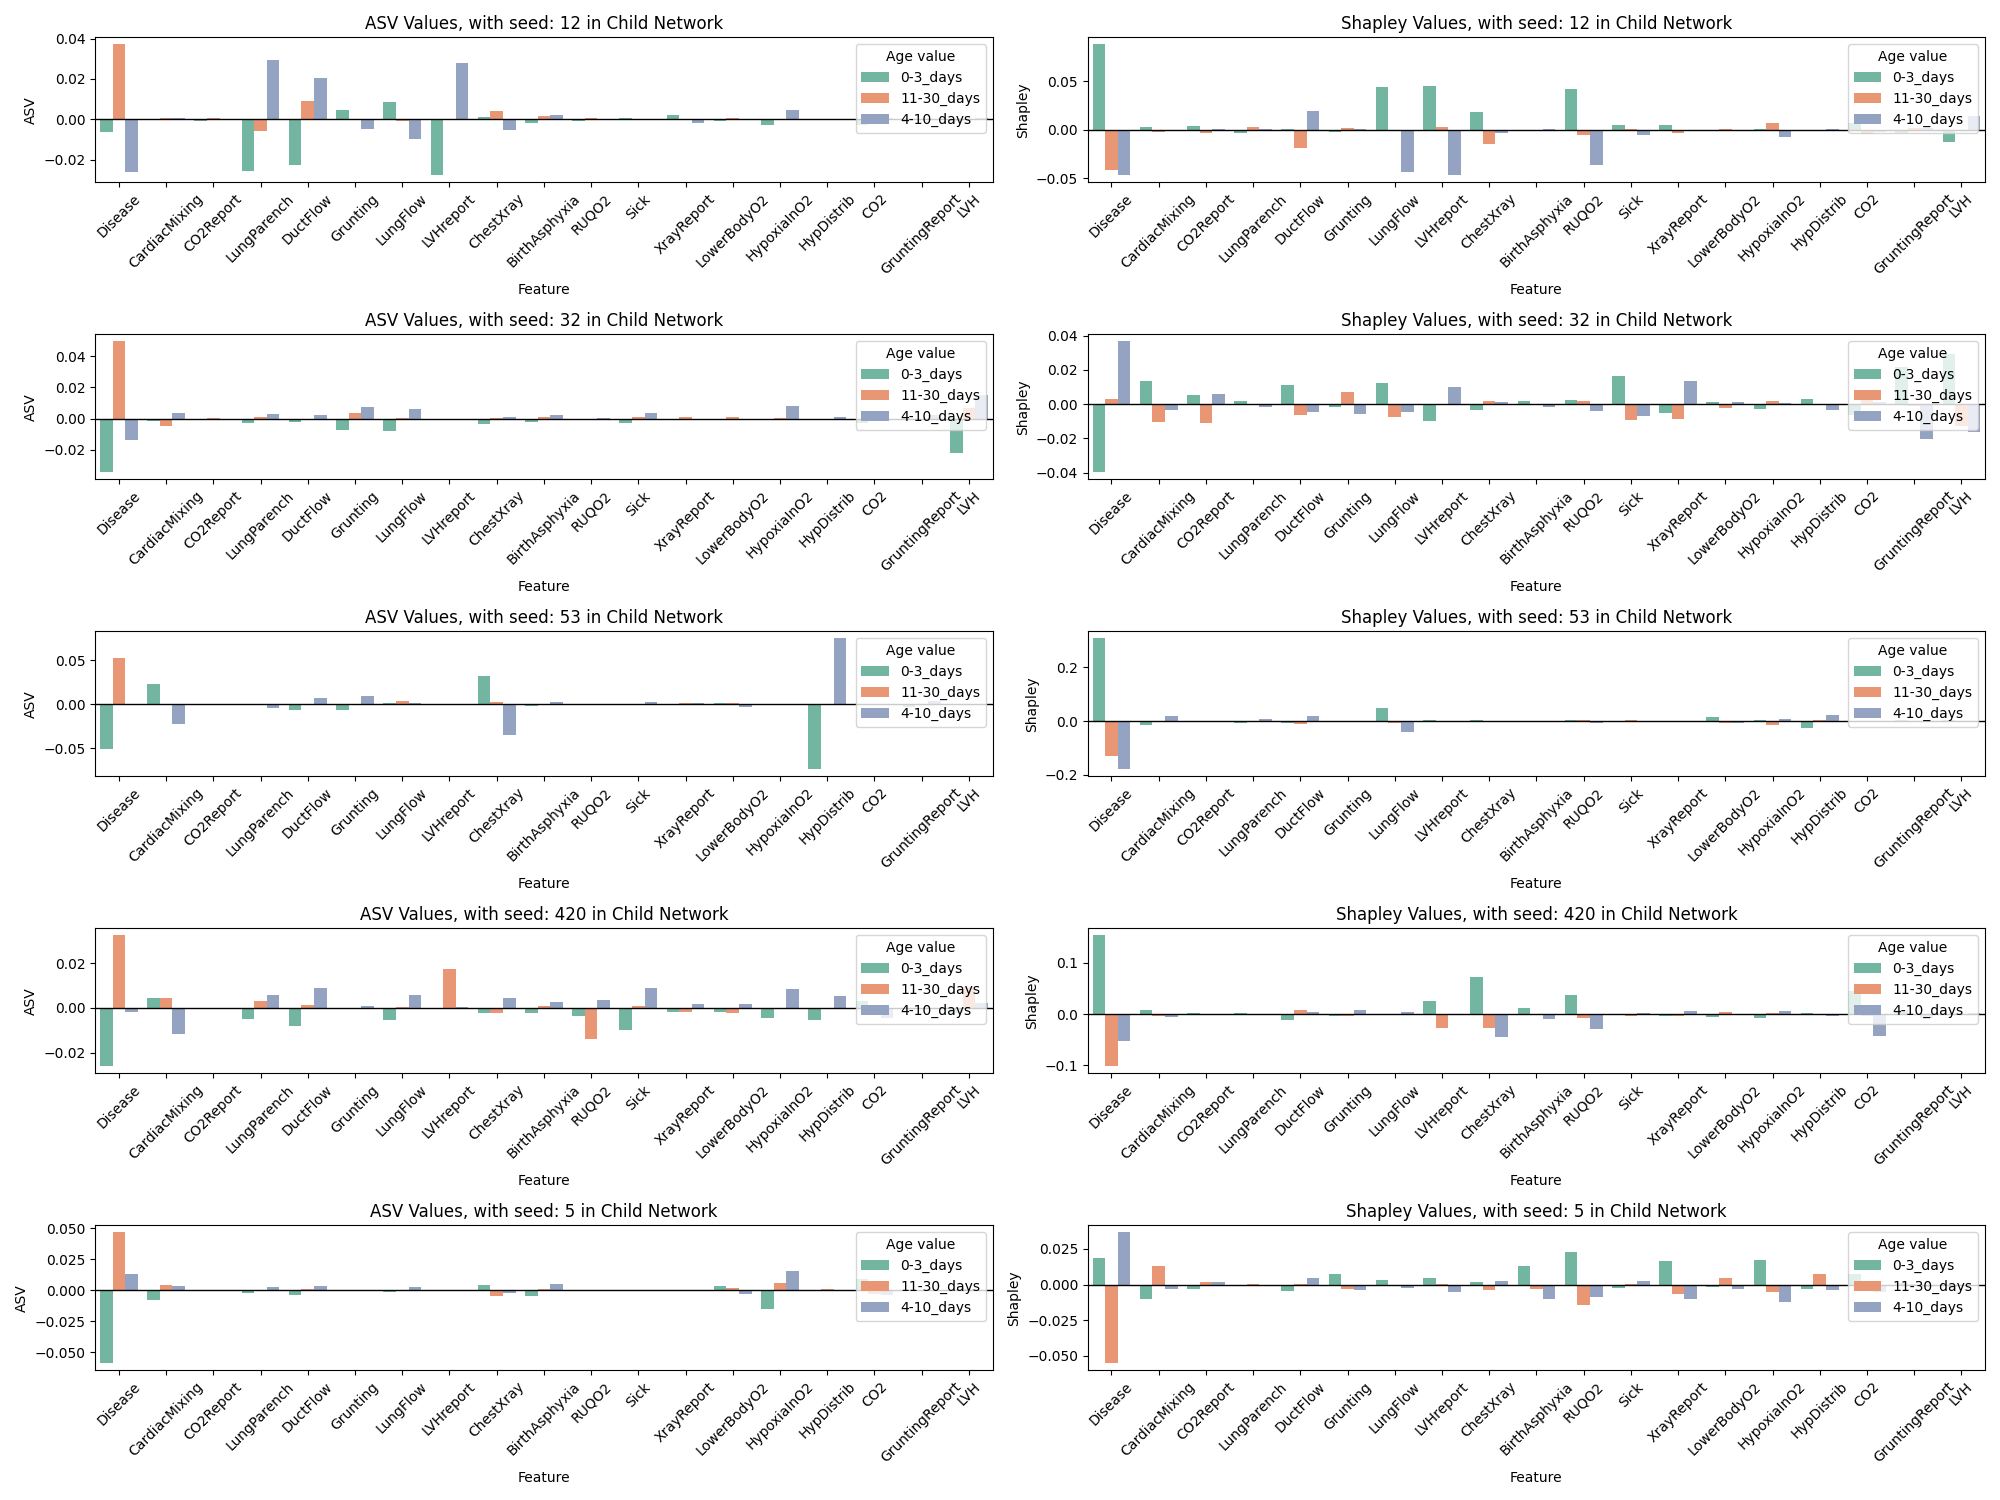
\includegraphics[scale=0.3]{img/asvResults/childMultipleSeedsASVandShapley.png}
    \caption{Comparación de los valores de ASV y Shapley para distintas seeds para la red Child}
    \label{fig:multipleSeedsASVvsShapleyChild}
\end{figure}

\begin{figure}[ht]
    \centering
    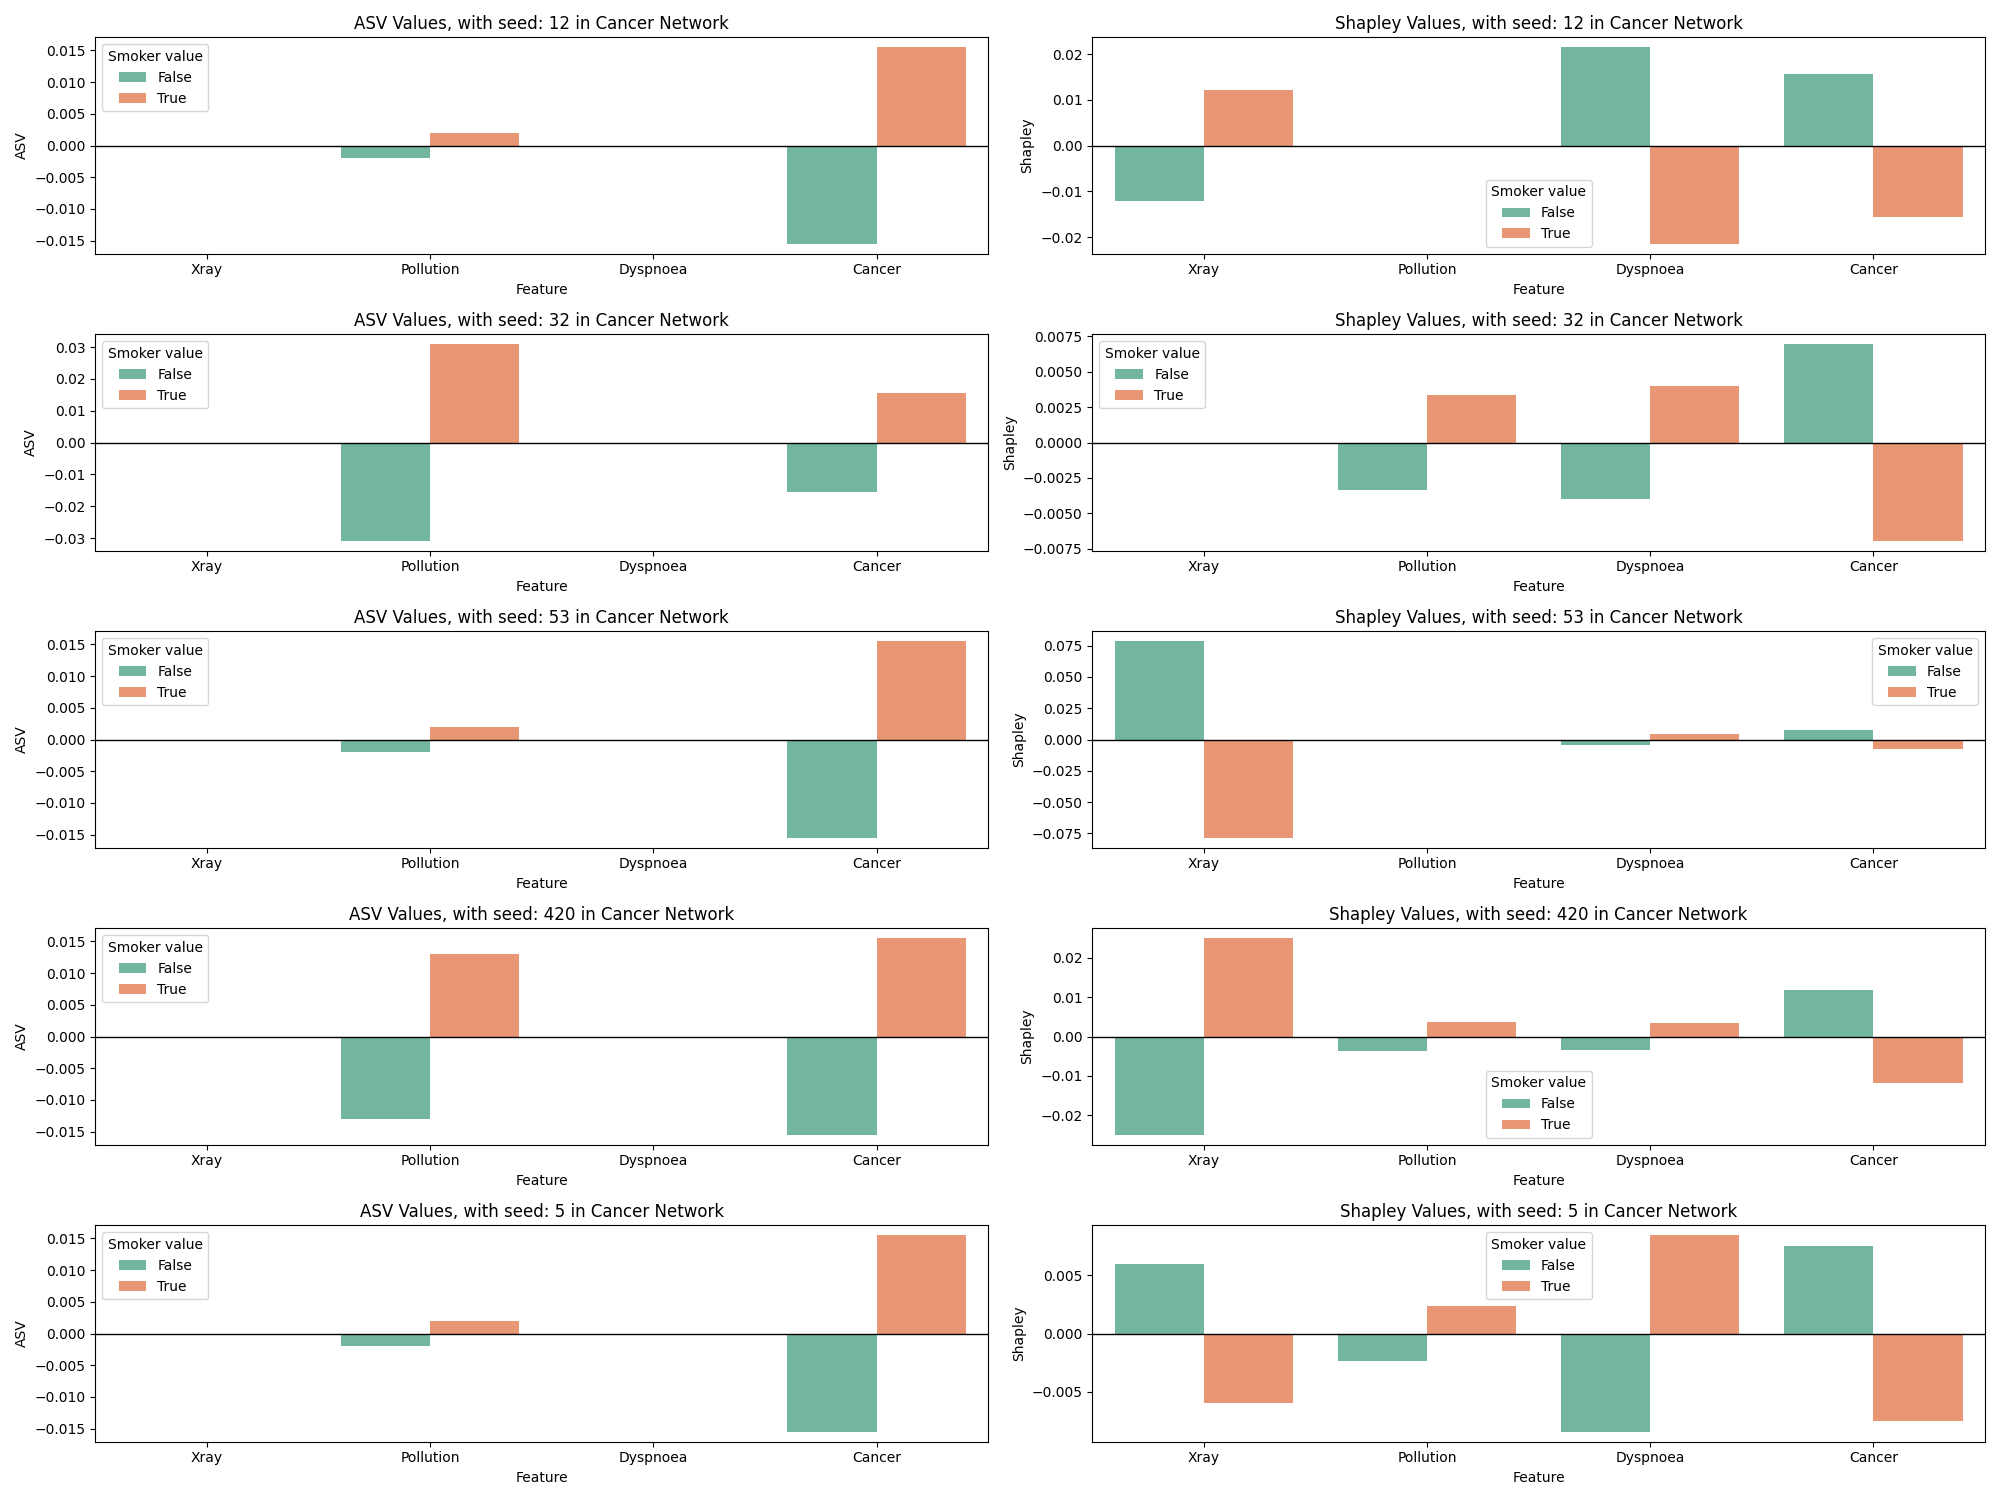
\includegraphics[scale=0.3]{img/asvResults/cancerMultipleSeedsASVandShapley.png}
    \caption{Comparación de los valores de ASV y Shapley para distintas seeds para la red Cancer}
    \label{fig:multipleSeedsASVvsShapleyCancer}
\end{figure}